\section{Homepage}

\begin{figure}[h!]
	\centering
	\begin{subfigure}[b]{0.3\textwidth}
		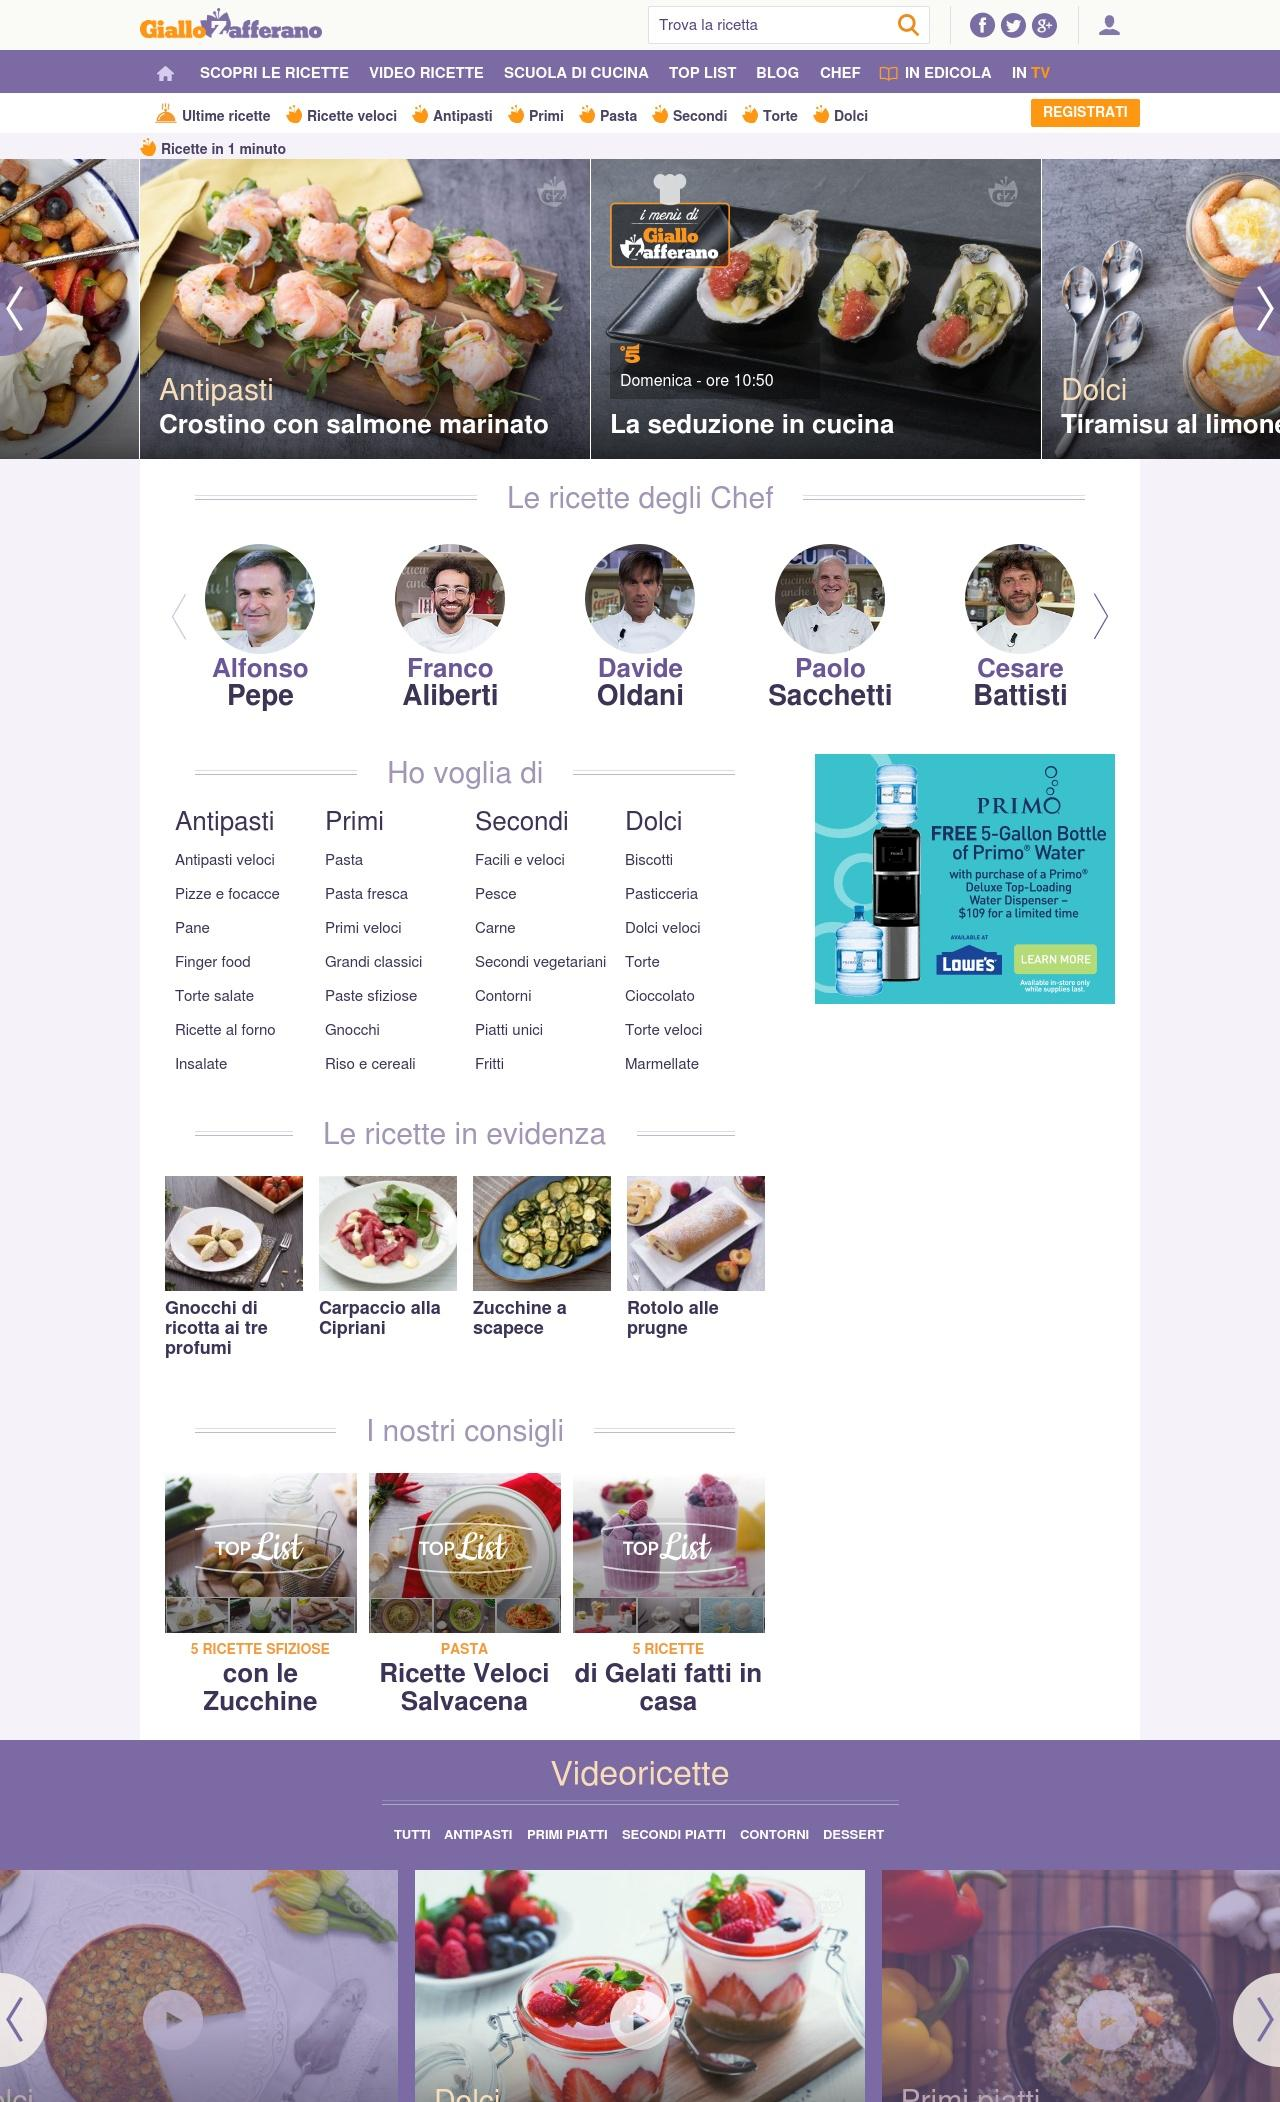
\includegraphics[scale=0.1]{images/homepage/homepage-1.jpeg}
		\subcaption{}
	\end{subfigure}
	\begin{subfigure}[b]{0.3\textwidth}
		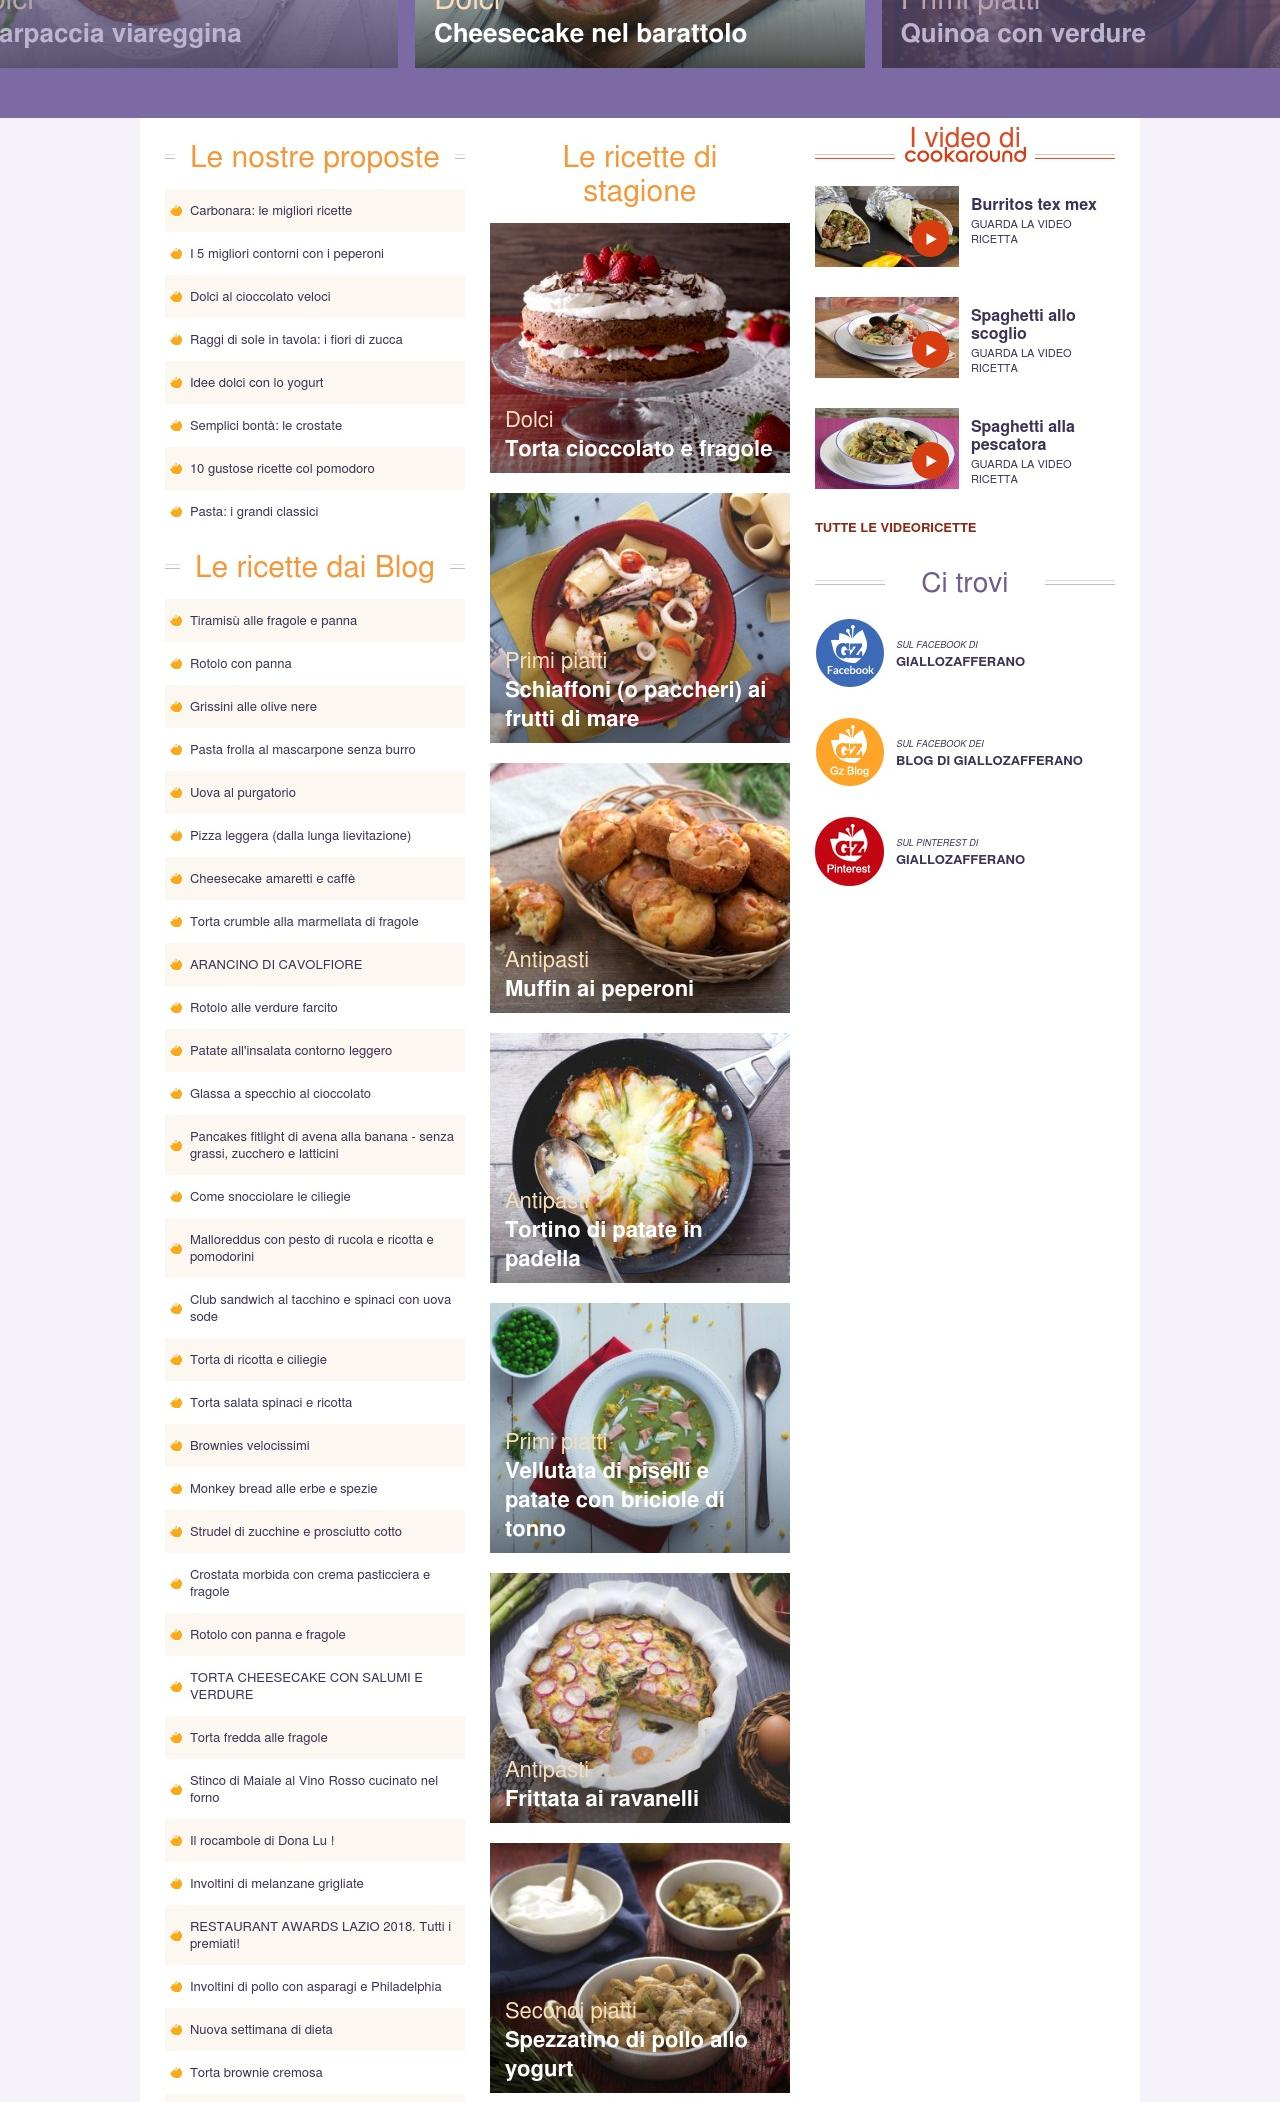
\includegraphics[scale=0.1]{images/homepage/homepage-2.jpeg}
		\subcaption{}
	\end{subfigure}
	\begin{subfigure}[b]{0.3\textwidth}
		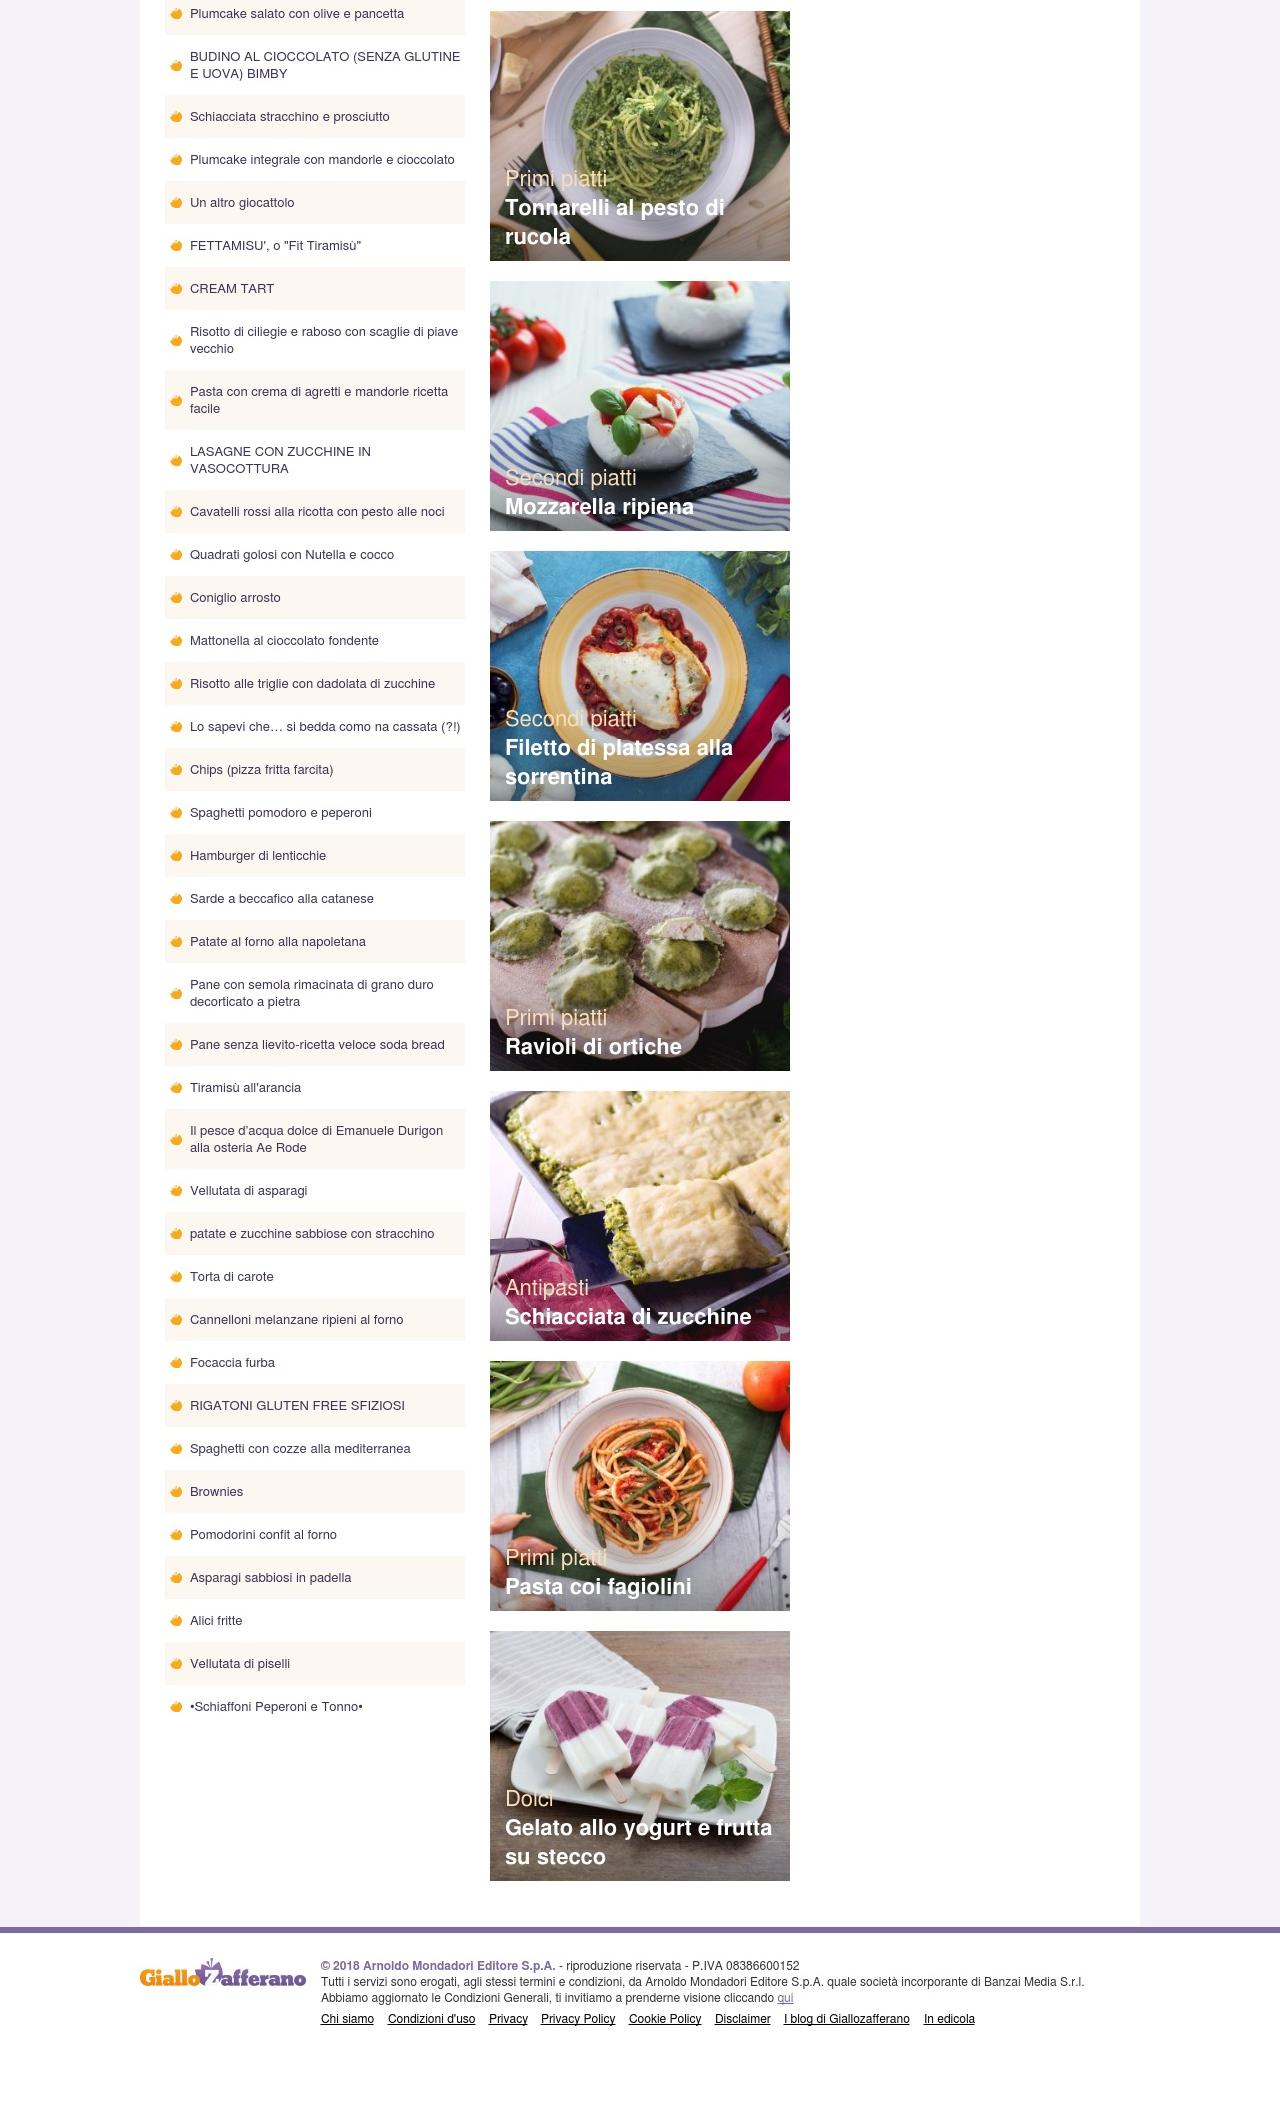
\includegraphics[scale=0.1]{images/homepage/homepage-3.jpeg}
		\subcaption{}
	\end{subfigure}
	\caption{Homepage (homepage-1,2,3.png) - https://www.giallozafferano.it}
	\label{fig:homepage}
\end{figure}


\subsection{Considerazioni generali}
L'homepage sta ad un sito web come la vetrina sta ad un negozio: essa ha infatti un ruolo introduttivo unico, in cui l'informazione deve essere fruibile nel modo più efficace possibile. Un buon design della homepage deve tener conto di quattro elementi principali:
\begin{itemize}
	\item Identità, del sito stesso o della compagnia/persona che rappresenta;
	\item Navigazione;
	\item Tempestività ed attenzione al contenuto;
	\item Strumenti, come la ricerca.
\end{itemize}
Il modo in cui l'importanza di questi elementi viene pesata dipende molto dalla natura del sito; l'homepage di giallozafferano è dominata dalla navigazione verso i contenuti : si vede subito come i riferimenti alle varie categorie di ricette siano disponibili immediatamente, sia nella barra di navigazione che nel corpo vero e proprio.

\subsection{Le 6 W}
Al fine di valutare come l'informazione viene presentata, si farà riferimento ai 6 assi informativi: Where, Who, Why, What, When, How; essi devono essere dati all'utente nel minor tempo possibile.

\subsubsection{Where} 

Domanda: \textit{"A quale sito sono arrivato? Che tipo di contenuto mi offre?"}

Come detto in precedenza, già nell'homepage notiamo una forte attenzione ai contenuti. Ciò è molto utile ad un utente che arriva per la prima volta nel sito, in quanto sin da subito capisce che si tratta di un sito collegato alla cucina; è probabile però che a primo impatto si possa pensare di essere arrivati nel sito di un ristorante: l'utilizzo di uno slide di immagini che occupa più della metà della parte superiore della pagina presenta foto di cibi, senza alcun riferimento al fatto che rimandano alla ricetta di quel piatto. Solo dopo aver superato l'impatto grafico iniziale, ci si accorge della parola \textit{ricette} che ricorre più volte, e si realizza di essere arrivati in un sito di ricette culinarie. 
Altro elemento che fa capire di essere in un sito il cui tema è la cucina è il nome, posto correttamente nell'angolo superiore sinistro della pagina (punto d'entrata della visualizzazione della pagina), nel quale \textbf{zafferano} richiama l'ingrediente principale del famoso risotto alla milanese.

\begin{figure}[h!]
	\centerline{
	
\includegraphics[scale=0.25]{images/homepage/header.png}}
	\caption{Header con logo (header.png)}
\end{figure}


\subsubsection{Who} 

Domanda: \textit{"Chi c'è dietro questo sito?"}

L'identità del creatore/possessore del sito non risulta totalmente chiara: sicuramente la presenza ben visibile del logo aiuta ad identificarlo se già lo si conosce, tuttavia per un utente che non ha mai sentito parlare del sito l'autore risulta ignoto e probabilmente rimarrà tale; in effetti, per trovare alcune informazioni a riguardo, è necessario scorrere fino alla fine della pagina (che come detto in precedenza è troppo lunga), fino ad arrivare nel footer, dove è scritto con un carattere molto piccolo il proprietario, \textit{Arnoldo Mondadori Editore S.p.A.}, al di sotto del quale è poi presente un link \textit{Chi siamo}, che porta ad una pagina che offre alcune informazioni aggiuntive riguardo non solo l'azienda, ma anche il team che lavora per il sito.
In sintesi dunque l'asse who non è ben specificato, poiché richiede troppo tempo per trovare risposta, cosa che l'utente non ha e che può portare ad un aumento dell'insoddisfazione.

\begin{figure}[h!]
	\centerline{
	
\includegraphics[scale=0.25]{images/homepage/footer.png}}
	\caption{Footer (footer.png)}
\end{figure}

\begin{figure}[h!]
	\centerline{
	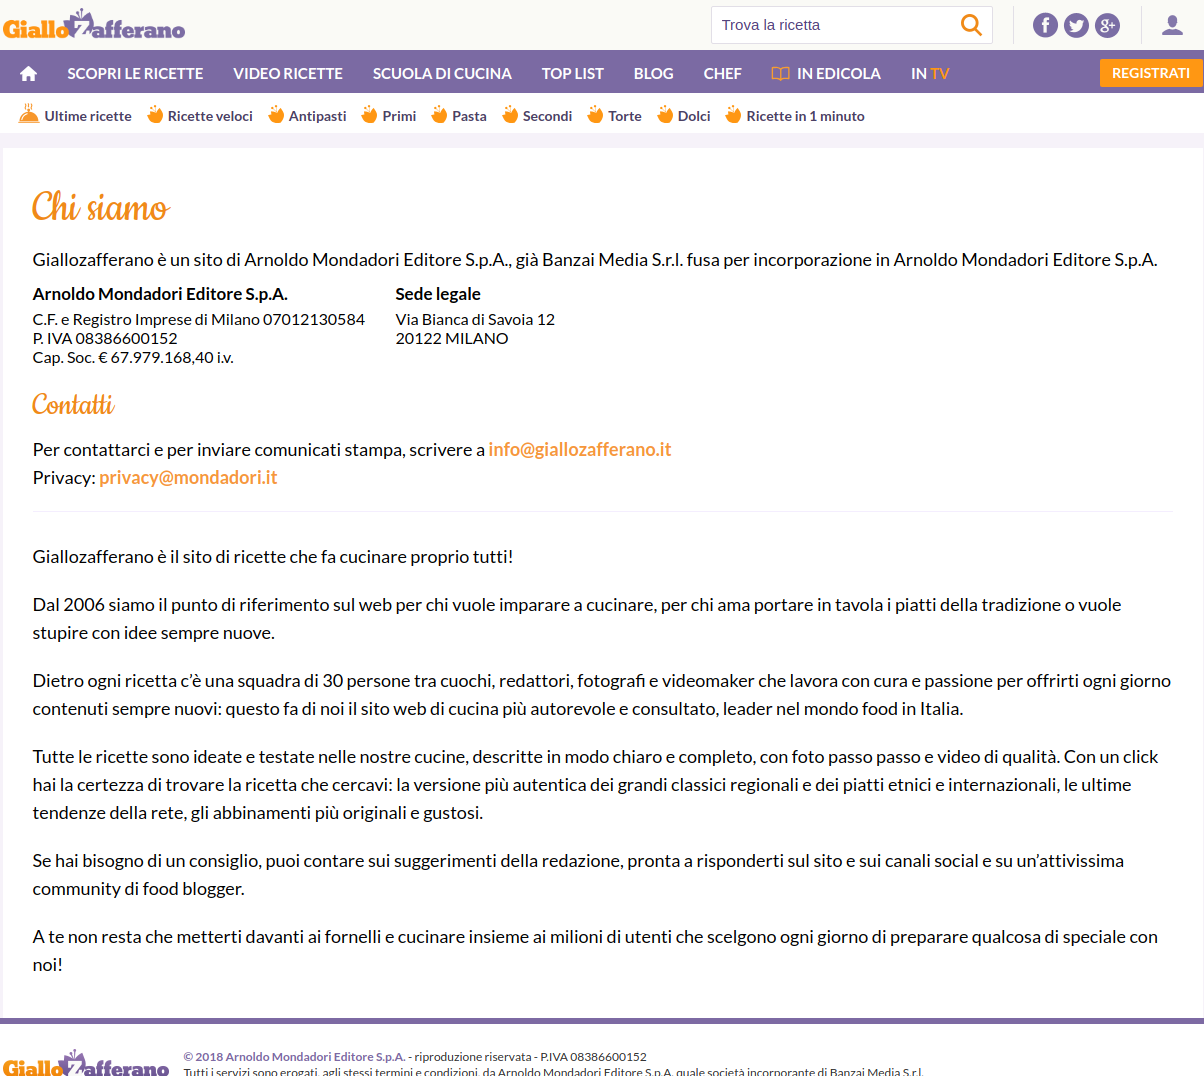
\includegraphics[scale=0.25]{images/chi-siamo.png}}
	\caption{Pagina "chi siamo" (chi-siamo.png) \newline- www.giallozafferano.it/staff/chisiamo.html}
\end{figure}

\newpage

\subsubsection{Why} 

Domanda: \textit{"Perché dovrei rimanere nel sito? Che benefici mi offre?"}

Il sito non dà esplicitamente dei motivi per cui un utente dovrebbe rimanerci, probabilmente perché si basa molto sulla propria fama (come specificato nell'analisi preliminare, esso è tra i più visitati al mondo nel settore cibo). Nonostante la fama conti, però, non è vantaggioso basarsi solo su di essa: nel web navigano persone con capacità e conoscenze diverse che il sito deve essere in grado di accogliere e "tenere" nel maggior numero possibile; ad esempio, un utente che non ha mai cercato ricette di cucina, potrebbe decidere di lasciare il sito perché non esperto del settore e perché non è in grado di valutare in breve tempo la qualità e l'affidabilità di giallozafferano, nonostante le numerose sezioni e i richiami agli chef che propone nella home. Per aumentare l'attrattiva, basterebbe un breve paragrafo di testo in cui esaltare i motivi del successo del sito, come ad esempio ciò che è scritto nella pagina "Chi siamo".

\newpage

\subsubsection{What} 

Domanda: \textit{"Che cosa offre il sito?"}

Come già detto, l'homepage è fortemente orientata al contenuto, che viene proposto più volte ed in maniera diversa. Il menù di navigazione (quello più in alto) principale presenta diverse voci che richiamano ciò che offre il sito, cioè le ricette, tuttavia è costituito da elementi poco chiari ed è necessario passarci sopra con il mouse per capire meglio a cosa portano. La presenza ricorrente della parola \textit{ricette}, in tutta la home, dà un'ulteriore conferma del contenuto del sito, assieme al sottomenù ed agli elenchi nella sezione \textit{Ho voglia di} (purtroppo tagliati in uno schermo con risoluzione 1920x1080, come si vede in \ref{fig:home_primo_pezzo}), i quali però richiamano parte del secondo menù di navigazione, il che ancora una volta rischia di creare confusione. 

\begin{figure}[h!]
	\centerline{
	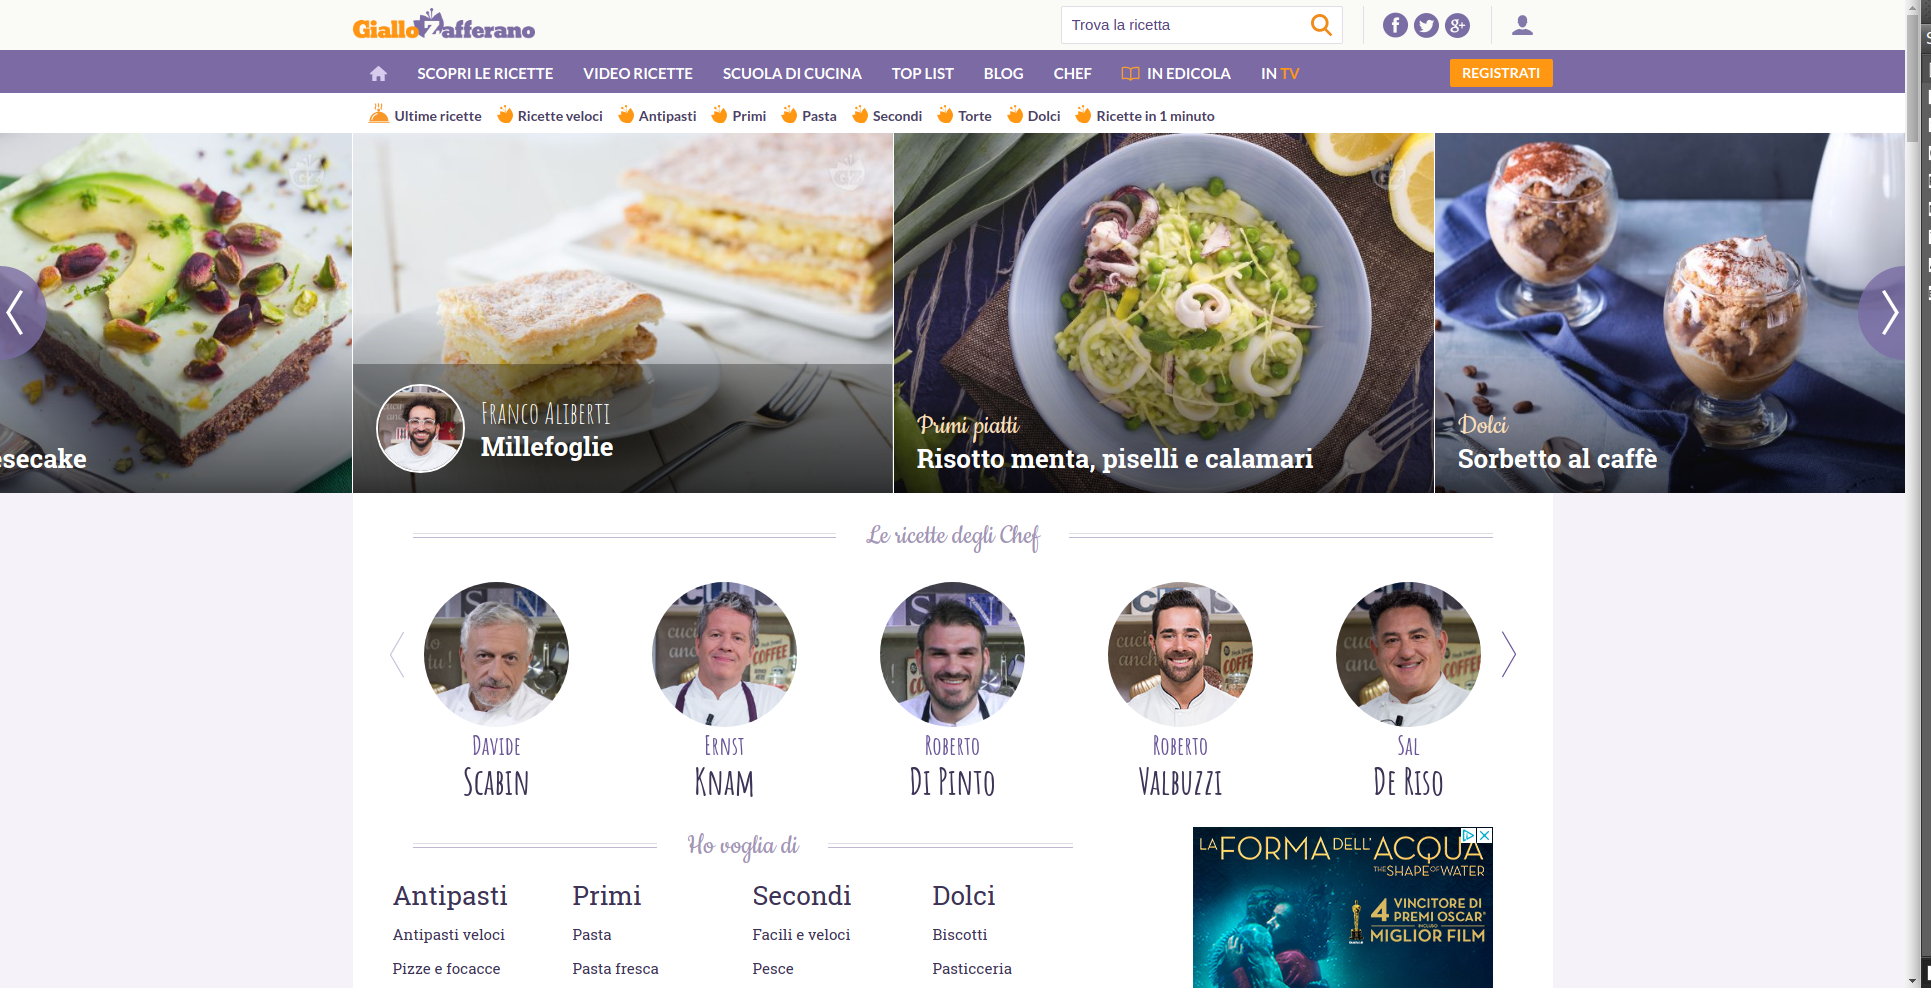
\includegraphics[scale=0.25]{images/home_primo_pezzo.png}}
	\caption{Homepage, prima schermata (home\textunderscore primo\textunderscore pezzo.png)}
	\label{fig:home_primo_pezzo}
\end{figure}


\subsubsection{When} 
\label{subsez:when}

Domanda: \textit{"Ciò che mi offre il sito è nuovo/aggiornato?"}

La homepage non dà alcun riferimento temporale. L'unica indicazione di novità sta nel secondo menù, nel quale compare la voce \textit{Ultime ricette} (vedi \ref{fig:secondo_menu}). Essa però non basta a dare un senso di aggiornamento continuo e novità al sito, è un elemento statico che non cambia nel tempo; cliccandoci sopra, inoltre, si arriva ad una pagina in cui vengono elencate le ultime ricette, senza però fornire alcuna data: l'intero sito dunque non riesce a soddisfare quest'asse sufficientemente.

\newpage

\subsubsection{How} 

Domanda: \textit{"Ho capito cosa mi offre. Come faccio ad arrivare a ciò che mi interessa?"}

La home fornisce diverse strade per raggiungere il contenuto, il che è un pregio, tuttavia sono disposte in modo confusionario; di seguito vengono analizzati in dettaglio i macro-componenti che racchiudono questi percorsi.

\paragraph{Primo menù di navigazione}
Il primo menù è abbastanza visibile ed è posto in alto, miglior posizione possibile. Le voci sono scritte in maiuscolo, cosa che diminuisce di circa il 10\% la leggibilità data la poca abitudine dell'utente medio a leggerlo.

\begin{figure}[h!]
	\centerline{
	
\includegraphics[scale=0.5]{images/primo_menu.png}}
	\caption{Primo menù di navigazione(primo\textunderscore menu.png)}
	\label{fig:primo_menu}
\end{figure}

\subparagraph{Voci}
\begin{itemize}
	\item \textbf{SCOPRI LE RICETTE} rimanda ad una pagina contenente tutte le ricette presenti nel sito divise per portata ed ha un sottomenù le cui voci sono le varie portate e rimandano alla stessa pagina, in cui però le ricette sono già filtrate in base alla voce scelta.
	\item \textbf{VIDEO RICETTE} ha un sottomenù identico al precedente e rimanda ad una pagina contente tutte le ricette aventi oltre ad una descrizione scritta, un video, divise per portata. Il fatto che questi primi due link rimandino ad una pagina così simile può però confondere l'utente, che potrebbe aspettarsi pagine completamente diverse: al momento dell'analisi, invece, le pagine risultano perfettamente identiche, le stesse ricette sono presentate in entrambe. In effetti ci si accorge che \textit{VIDEO RICETTE} non è una pagina a parte, bensì una sotto-pagina di \textit{SCOPRI LE RICETTE}! Personalmente dunque ritengo la scelta di riservarvi una voce di menù controproducente, sarebbe meglio invece usarla come filtro di ricerca o come voce del sottomenù di \textit{SCOPRI LE RICETTE};
	\item \textbf{SCUOLA DI CUCINA} è un'altra voce che può creare confusione: l'insegnamento della cucina non comprende anche le ricette? Solo passandoci sopra  con il mouse e facendo comparire il sottomenù ci si accorge che sono comprese solo tecniche e ricette "generali", cioè non legate ad uno specifico piatto, come ad esempio pulire la verdura,  preparare salse basilari ecc...
	\item \textbf{TOP LIST}: ancora una volta non è ben chiaro a cosa si riferisca la voce; innanzitutto l'utilizzo dell'inglese non è appropriato in un sito italiano, soprattutto considerando la grande varietà di utenti a cui si rivolge: ad esempio, molto probabilmente un anziano non ha idea di cosa voglia dire di preciso. 
	Comunque, anche ammesso che un utente conosca l'inglese, tale voce rimane vaga: lista dei migliori? E' intuibile che ci si sta riferendo alle migliori ricette, ma non è assolutamente banale.
	\item \textbf{BLOG} rimanda al blog collegato al sito (ma esterno), come ci si aspetta.
	\item \textbf{CHEF} rimanda alla pagina delle ricette ideate dagli chef che lavorano per il sito, mentre ci si aspetterebbe un semplice elenco di essi.
	\item \textbf{IN EDICOLA} rimanda ad una pagina informativa riguaro la rivista collegata al sito, come ci si aspetta.
	\item \textbf{IN TV} rimanda ad una pagina il cui titolo è \textit{"I menù di giallozafferano"}, la cui natura è inaspettata e non molto chiara; probabilmente infatti un utente si aspetta di trovare una pagina informativa come quella a cui rimanda la voce precedente, invece trova dei contenuti totalmente diversi sia strutturalmente che concettualmente.
\end{itemize}


\subparagraph{Sottomenù}

Le prime tre voci del menù appena descritto hanno un comportamento dinamico: quando il cursore ci passa sopra, compare un sottomenù: il fatto che ciò accada con solo una parte delle voci è un difetto, in quanto rende la struttura del menù poco prevedibile. In ogni caso, i sottomenù a tendina sono facilmente navigabili, in quanto viene lasciato un margine abbastanza ampio tra la parola e la dimensione effettiva del pulsante; il fatto che si espandano verticalmente inoltre è una buona cosa e da preferire rispetto ad un elenco orizzontale. Un difetto è il non essere \textit{fault tollerant}, cioè non appena il cursore esce dal sottomenù, questo scompare.


\begin{figure}[h!]
	\centering
	\begin{subfigure}[b]{0.3\textwidth}
		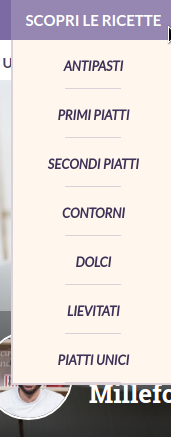
\includegraphics[scale=0.5]{images/sottomenu-1.png}
		\subcaption{}
	\end{subfigure}
	\begin{subfigure}[b]{0.3\textwidth}
		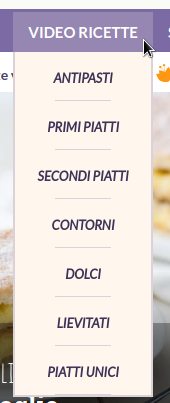
\includegraphics[scale=0.5]{images/sottomenu-2.png}
		\subcaption{}
	\end{subfigure}
	\begin{subfigure}[b]{0.3\textwidth}
		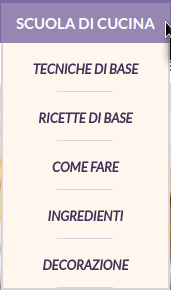
\includegraphics[scale=0.5]{images/sottomenu-3.png}
		\subcaption{}
	\end{subfigure}
	\caption{I 3 sottomenù (sottomenu-1.png, sottomenu-2.png, sottomenu-3.png)}
\end{figure}



\paragraph{Secondo menù di navigazione}

Il secondo menù è posto appena sotto il primo e riporta molti riferimenti già definiti in precedenza.

\begin{figure}[h!]
	\centerline{
	
\includegraphics[scale=0.5]{images/secondo-menu.png}}
	\caption{Secondo menù di navigazione (secondo-menu.png)}
	\label{fig:secondo_menu}
\end{figure}

\subparagraph{Voci}

\begin{itemize}
	\item \textbf{Ultime ricette} Come detto in \ref{subsez:when}, rimanda alla pagina con le ultime ricette.
	\item \textbf{Ricette veloci - Antipasti - Primi - Pasta - Secondi - Torte - Dolci} Si comportano come le voci dei sottomenù delle prime due voci del primo menù di navigazione, quindi rimandano alla pagina delle ricette, visualizzando solo la categoria scelta: si riconferma la ridondanza e la conseguente confusione di link ripetuti inutilmente.
	\item \textbf{Ricette in un minuto} Tale voce ha un comportamento completamente diverso dalle altre: rimanda alla pagina https://funtip.giallozafferano.it/, che si presenta totalmente diversa dalle altre, senza alcun menù di navigazione, ad esempio.
\end{itemize}

\paragraph{Riferimenti nel corpo}

L'intero contenuto della pagina presenta ulteriori link a categorie di ricette o ricette singole. Precisamente, ci sono 9 componenti diverse che li racchiudono, che tuttavia ometto di descrivere in quanto vale quello che è stato detto per i vari menù, cioè il fatto che creano solamente un senso di confusione e ridondanza
(sono visibili nella figura \ref{fig:homepage}, nel corpo della pagina).


